La figure suivante (figure \ref{diagramme_sequence}) indique le déroulement du remplissage de la base de données via les fichiers csv.

\begin{figure}[H]
	\centering
	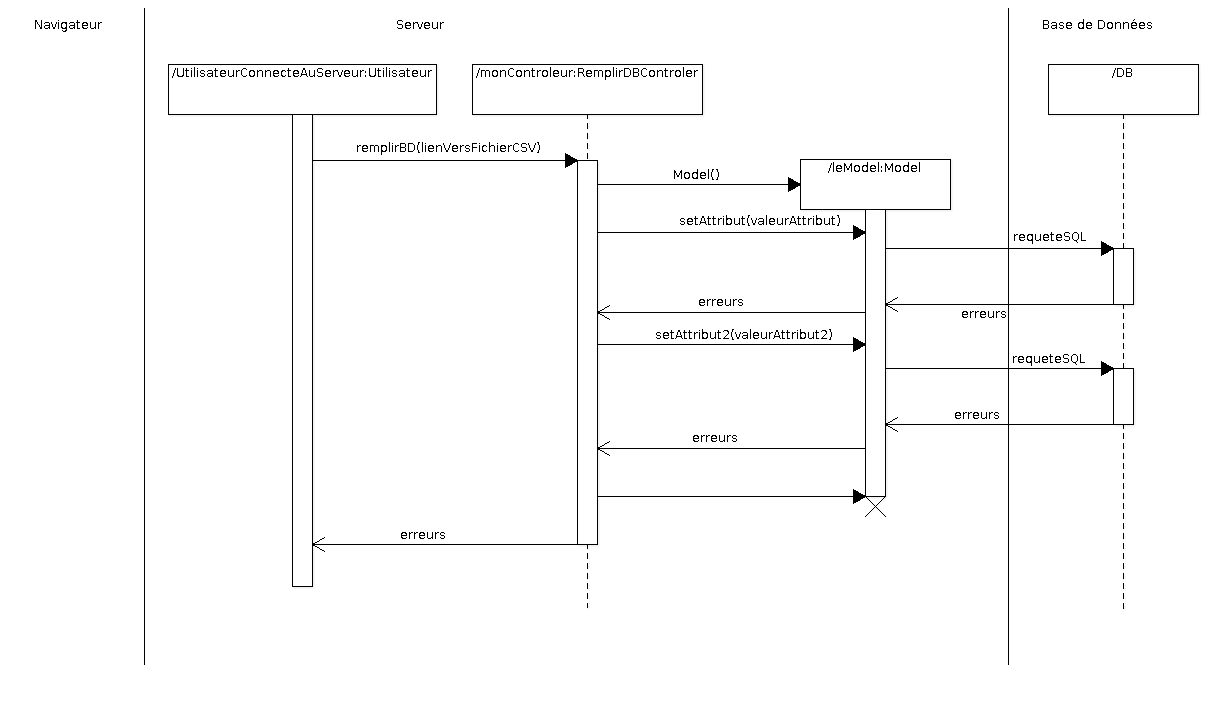
\includegraphics[scale=0.3]{diagrammeSequence/images/diagrammeSequence}
	\caption{Diagramme de séquence système pour le remplissage de la base de données}	
	\label{diagramme_sequence}
\end{figure}
	
%\newpage
La figure suivante (figure \ref{diagramme_sequence_2}) montre les actions effectuées lors d'une interaction entre l'utilisateur et l'IHM.

\begin{figure}[H]
	\centering
	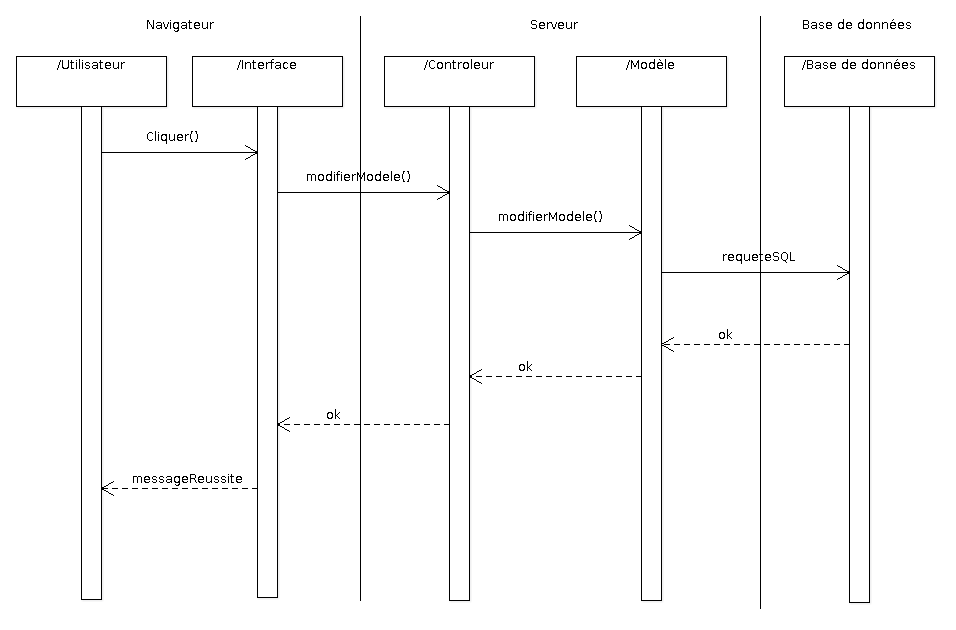
\includegraphics[scale=0.3]{diagrammeSequence/images/diagrammeSequenceAction}
	\caption{Diagramme de séquence système pour une interaction de l'utilisateur}
	\label{diagramme_sequence_2}
\end{figure}